\section{Optimization} \label{sec:factorial}
%\begin{tcolorbox}
%	Die Fakultät einer Zahl $n\in\mathbb N_0$ is definiert als
%	\begin{equation*}
%		n!=1\cdot 2\cdot 3\cdot\ldots\cdot \left(n-1\right)\cdot n,
%	\end{equation*}
%	wobei $0!=1$ und $1!=1$.
%	Sind $n$ Elemente auf $n$ Plätze zu verteilen, so gibt es dafür $n!$ Möglichkeiten.
%\end{tcolorbox}
\begin{exercise}
	We want to build rectangular garden, where one edge is given by a wall.
	The remaining three edges of the garden are bounded by a fence of length 64 meters.
	We want to find the length of the edges $x$ and $y$ of the rectangular fence that maximize the surrounded area.\\
\begin{minipage}{0.66\textwidth}
	\begin{tasks}
		\task What result do you expect for $x$ and $y$?
		\task Find a function $f(x)$ that describes the surrounded area.
		\task Compute the optimal values for $x$ and $y$.
		\task What if the fence has length $a$ instead?
	\end{tasks}
\end{minipage}\hfill
\begin{minipage}{0.33\textwidth}
	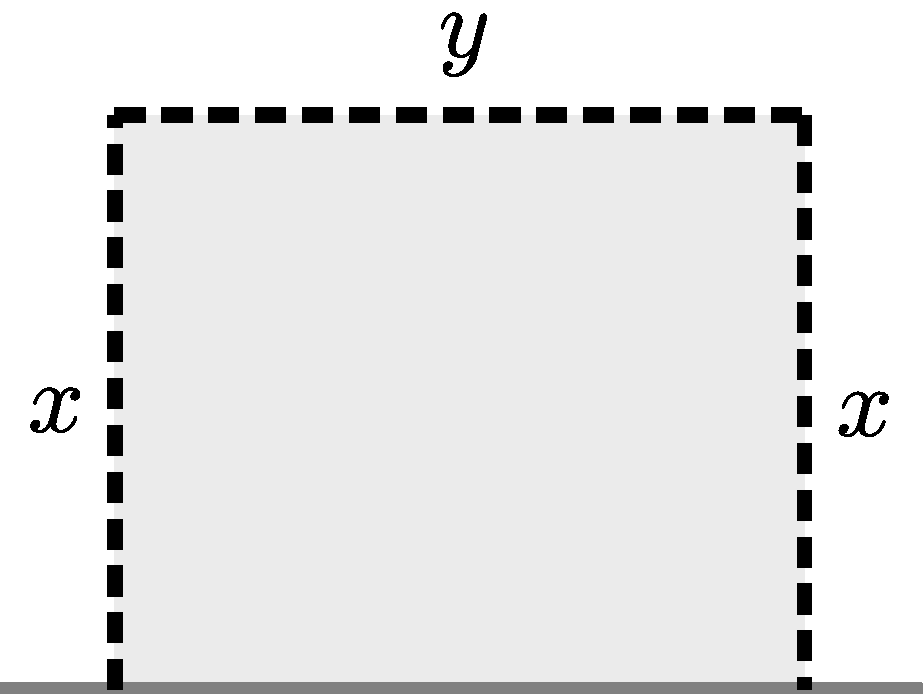
\includegraphics[width=0.9\textwidth]{images/fence}
\end{minipage}
\end{exercise}
\begin{comment}
\begin{solution*}
	\phantom{text}
	\begin{tasks}
		\task The enclosure wants to ``use'' as much of the wall as it can.
		Thus we expect the edge parallel to the wall to be a bit larger than the the two edges orthogonal to the wall.
		\task $f(x)=x\cdot\left(64-2x\right)$
		\task Plug in $a=64$ below.
		\task The area of the garden is given by $x\cdot y$ with the \textbf{constraint} $2x+y=a$.
		We use the constraint to replace $y$.
		Thereby we obtain the target function
		\begin{equation*}
			f\left(x\right)=x\cdot\left(a-2x\right)
		\end{equation*}
		for the surrounded area.
		If we set the derivative
		\begin{equation*}
			f^\prime\left(x\right)=-2x+\frac{a}{4}.
		\end{equation*}
		to zero and solve for $x$, we obtain $x_0=\frac{a}{4}$.
		This is indeed a maximum since
		\begin{equation*}
			f^{\prime\prime}\left(x\right)=-2
		\end{equation*}
		is negative at every $x$ and in particular at $x_0$.
	\end{tasks}
\end{solution*}
\end{comment}
\begin{minipage}{0.8\textwidth}
	\begin{exercise}
		We want to build a window with a semicircle on top (see image).
		If there is 12 meters of framing materials,
		what must be the dimensions of the window to let in the most light
		(i.e. maximal area)?
	\end{exercise}
\end{minipage}\hfill
\begin{minipage}{0.15\textwidth}
	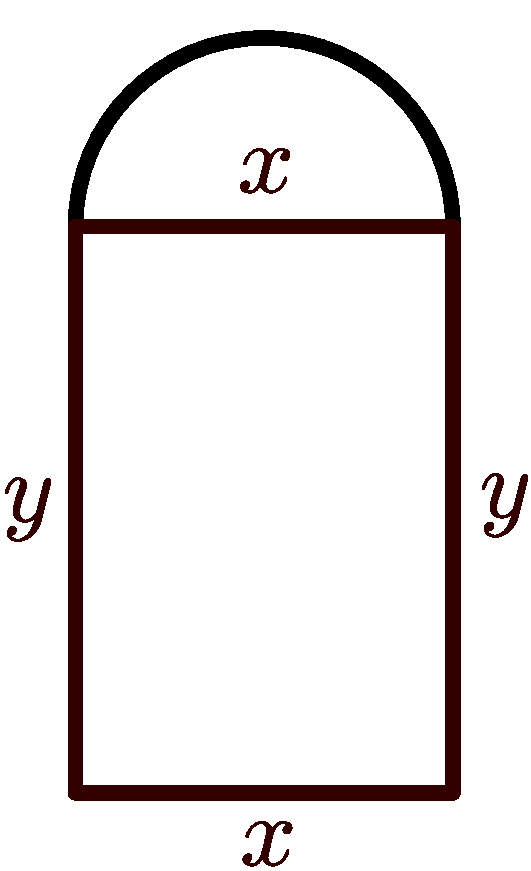
\includegraphics[width=\textwidth]{images/window}
\end{minipage}\\
\begin{solution*}
	The formulas for the perimeter (Umfang) and the area are given by
	\begin{equation*}
		\left(1+\frac{\pi}{2}\right)x+2y
		\quad\text{and}\quad
		\frac{\pi}{8}x^2+xy,
	\end{equation*}
	respectively.
	Since the perimeter equals 12 meters, we set the first equation equal to 12 and solve for $y$.
	We obtain
	\begin{equation*}
		y=-\frac{\pi+2}{4}x^2+6
	\end{equation*}
	and plug this into the equation for the area, which becomes our target function
	\begin{equation*}
		f\left(x\right)=-\frac{\pi+4}{8}x^2+6x.
	\end{equation*}
	To find the critical point(s), we set the derivative
	\begin{equation*}
		f^{\prime}\left(x\right)=-\frac{\pi+4}{4}x+6
	\end{equation*}
	equal to zero and solve for $x$.
	We get
	\begin{equation*}
		x_0=\frac{24}{\pi+4}.
	\end{equation*}
	This is indeed a maximum, since
	\begin{equation*}
		f^{\prime\prime}\left(x\right)=-\frac{\pi+4}{4}
	\end{equation*}
	is negative at every $x$ and in particular at $x_0$.
\end{solution*}